\documentclass{anstrans}

%%%% packages and definitions (optional)
\usepackage{graphicx} % allows inclusion of graphics
\usepackage{booktabs} % nice rules (thick lines) for tables
\usepackage{microtype} % improves typography for PDF
\usepackage{algorithm}
\usepackage{algorithmic}
\usepackage{mathtools}
\usepackage{amsmath}
\usepackage{fancyhdr} 
\usepackage{subfigure}



%%%%%%%%%%%%%%%%%%%%%%%%%%%%%%%%%%%
\title{Heat Source Characterization In A TREAT Fuel Particle Using Coupled Neutronics Binary Collision Monte-Carlo Calculations}
\author{Sebastian Schunert$^1$, Daniel Schwen$^1$, Pedram Ghassemi$^2$, Benjamin Baker$^1$, Adam Zabriskie$^1$, Javier Ortensi$^1$, Yaqi Wang$^1$, Frederick Gleicher$^1$, Mark DeHart$^1$, Richard Martineau$^1$}
\institute{$^1$Idaho National Laboratory, Nuclear Science \&Technology Directorate, Idaho Falls, ID\\
               $^2$Department of Nuclear Engineering, North Carolina State University, Raleigh, NC}

\email{sebastian.schunert@inl.gov}

\renewcommand\headrule{} % remove underline in the header
\setcounter{secnumdepth}{1}
\renewcommand{\thesection}{\Roman{section}.}
\renewcommand{\thesubsection}{\arabic{subsection}.}
\renewcommand{\thesubsubsection}{\Alph{subsubsection}.}
\makeatletter
\renewcommand*{\@seccntformat}[1]{\csname the#1\endcsname\hspace{1mm}}
\makeatother

%%%% Header
\pagestyle{fancy}
\fancyhf{}
\fancyhead[L]{\fontsize{9}{9} \itshape
M\&C 2017 - International Conference on Mathematics \& Computational Methods Applied to Nuclear Science \& Engineering,
\\ Jeju, Korea, April 16-20, 2017, on USB (2017)
}

%  various packages that you may wish to activate for usage
\usepackage{graphicx}
\usepackage{tabls}
\usepackage{afterpage}
\usepackage{amsmath}
\usepackage{amsfonts}
\usepackage{amssymb}
\usepackage{amstext}
\usepackage{amsbsy}
\usepackage{epsfig}
%\usepackage{cites}
\usepackage{epsf}
\usepackage{float} %utiliser H pour forcer � mettre l'image o� on ve

\usepackage{array}
{\usepackage{color}}
\usepackage[section]{placeins} % force � mettre l'image o� on veut
\usepackage{lscape} %utilisation du mode paysage
\usepackage{xspace}

%\usepackage[pdftex,bookmarks=true]{hyperref}
\usepackage{url}
\usepackage{verbatim}
%\usepackage[all]{hypcap}

\usepackage[labelsep=quad]{caption} % needed by the breakalgo environment

\usepackage{ifthen}
%\usepackage{subfig}

\usepackage{algorithmic}
\usepackage{algorithm}
\usepackage{listings}
\usepackage[noprefix]{nomencl}  % for nomenclature
%\usepackage[intoc]{nomencl}  % for nomenclature

%\usepackage{notebook2e, latexsym}
%
% de dk:
%
%%\usepackage[dvips]{epsfig}
%%\usepackage[dvips]{graphicx}
%%\usepackage{comment}
%%\usepackage{floatfig}
%%\usepackage{lscape}
%%\usepackage{landscape}
%%\usepackage{graphics}
%%\usepackage{hhline}[]
%%\usepackage{latexsym}
%%\usepackage{tabularx}[]
%%\usepackage{layout}
%
% de btp:
%
%%\usepackage{fancyheadings}
%%\usepackage{minitoc}
\usepackage{rotating}
%% \usepackage{rotate}
\usepackage{subfigure}
%%\usepackage{mathaccent}
%%\usepackage{isolatin1}
%
%%\usepackage{xspace}
%%\usepackage{longtable}
%%\usepackage{caption2}
%%\usepackage{ifthen}
%
\usepackage{mathpazo}
\usepackage{hyperref}

%
%=================================================================================================
% new commands
% +++++++++++++++++++++++++++++++++++++++++++++++++++++++++++++++++++++++++++++++++++++++++++++++++
\newcommand{\nc}{\newcommand}
%
% Ways of grouping things
%
\newcommand{\bracket}[1]{\left[ #1 \right]}
\newcommand{\bracet}[1]{\left\{ #1 \right\}}
\newcommand{\fn}[1]{\left( #1 \right)}
\newcommand{\ave}[1]{\left\langle #1 \right\rangle}
%
% Derivative forms
%
\newcommand{\dx}[1]{\,d#1}
\newcommand{\dxdy}[2]{\frac{\partial #1}{\partial #2}}
\newcommand{\dxdt}[1]{\frac{\partial #1}{\partial t}}
\newcommand{\dxdz}[1]{\frac{\partial #1}{\partial z}}
\newcommand{\dfdt}[1]{\frac{\partial}{\partial t} \fn{#1}}
\newcommand{\dfdz}[1]{\frac{\partial}{\partial z} \fn{#1}}
\newcommand{\ddt}[1]{\frac{\partial}{\partial t} #1}
\newcommand{\ddz}[1]{\frac{\partial}{\partial z} #1}
\newcommand{\dd}[2]{\frac{\partial}{\partial #1} #2}
\newcommand{\ddx}[1]{\frac{\partial}{\partial x} #1}
\newcommand{\ddy}[1]{\frac{\partial}{\partial y} #1}
%
% Vector forms
%
%\renewcommand{\vec}[1]{\ensuremath{\stackrel{\rightarrow}{#1}}}
%\renewcommand{\div}{\ensuremath{\vec{\nabla} \cdot}}
%\newcommand{\grad}{\ensuremath{\vec{\nabla}}}

\renewcommand{\div}{\vec{\nabla}\! \cdot \!}
\newcommand{\grad}{\vec{\nabla}}
\newcommand{\oa}[1]{\fn{\frac{1}{3}\hat{\Omega}\!\cdot\!\overrightarrow{A_{#1}}}}

%
% Equation beginnings and endings
%
\newcommand{\bea}{\begin{eqnarray}}
\newcommand{\eea}{\end{eqnarray}}
\newcommand{\be}{\begin{equation}}
\newcommand{\ee}{\end{equation}}
\newcommand{\beas}{\begin{eqnarray*}}
\newcommand{\eeas}{\end{eqnarray*}}
\newcommand{\bdm}{\begin{displaymath}}
\newcommand{\edm}{\end{displaymath}}
%
% Equation punctuation
%
\newcommand{\pec}{\hspace{0.25in},}
\newcommand{\pep}{\hspace{0.25in}.}
\newcommand{\pev}{\hspace{0.25in}}
%
% Equation labels and references, figure references, table references
%
\newcommand{\LEQ}[1]{\label{eq:#1}}
\newcommand{\EQ}[1]{Eq.~(\ref{eq:#1})}
\newcommand{\EQS}[1]{Eqs.~(\ref{eq:#1})}
\newcommand{\REQ}[1]{\ref{eq:#1}}
\newcommand{\LFI}[1]{\label{fi:#1}}
\newcommand{\FI}[1]{Fig.~\ref{fi:#1}}
\newcommand{\RFI}[1]{\ref{fi:#1}}
\newcommand{\LTA}[1]{\label{ta:#1}}
\newcommand{\TA}[1]{Table~\ref{ta:#1}}
\newcommand{\RTA}[1]{\ref{ta:#1}}

%
% List beginnings and endings
%
\newcommand{\bl}{\bss\begin{itemize}}
\newcommand{\el}{\vspace{-.5\baselineskip}\end{itemize}\ess}
\newcommand{\benu}{\bss\begin{enumerate}}
\newcommand{\eenu}{\vspace{-.5\baselineskip}\end{enumerate}\ess}
%
% Figure and table beginnings and endings
%
\newcommand{\bfg}{\begin{figure}}
\newcommand{\efg}{\end{figure}}
\newcommand{\bt}{\begin{table}}
\newcommand{\et}{\end{table}}
%
% Tabular and center beginnings and endings
%
\newcommand{\bc}{\begin{center}}
\newcommand{\ec}{\end{center}}
\newcommand{\btb}{\begin{center}\begin{tabular}}
\newcommand{\etb}{\end{tabular}\end{center}}
%
% Single space command
%
%\newcommand{\bss}{\begin{singlespace}}
%\newcommand{\ess}{\end{singlespace}}
\newcommand{\bss}{\singlespacing}
\newcommand{\ess}{\doublespacing}
%
%---New environment "arbspace". (modeled after singlespace environment
%                                in Doublespace.sty)
%   The baselinestretch only takes effect at a size change, so do one.
%
\def\arbspace#1{\def\baselinestretch{#1}\@normalsize}
\def\endarbspace{}
\newcommand{\bas}{\begin{arbspace}}
\newcommand{\eas}{\end{arbspace}}
%
% An explanation for a function
%
\newcommand{\explain}[1]{\mbox{\hspace{2em} #1}}
%
% Quick commands for symbols
%
\newcommand{\half}{\frac{1}{2}}
\newcommand{\third}{\frac{1}{3}}
\newcommand{\twothird}{\frac{2}{3}}
\newcommand{\fourth}{\frac{1}{4}}
\newcommand{\mdot}{\dot{m}}
\newcommand{\ten}[1]{\times 10^{#1}\,}
\newcommand{\cL}{{\cal L}}
\newcommand{\cD}{{\cal D}}
\newcommand{\cF}{{\cal F}}
\newcommand{\cE}{{\cal E}}
\renewcommand{\Re}{\mbox{Re}}
\newcommand{\Ma}{\mbox{Ma}}
%
% Inclusion of Graphics Data
%
%\input{psfig}
%\psfiginit
%
% More Quick Commands
%
\newcommand{\bi}{\begin{itemize}}
\newcommand{\ei}{\end{itemize}}
\newcommand{\ben}{\begin{enumerate}}
\newcommand{\een}{\end{enumerate}}
\newcommand{\dxi}{\Delta x_i}
\newcommand{\dyj}{\Delta y_j}
\newcommand{\ts}[1]{\textstyle #1}


\newcommand{\bu}{\boldsymbol{u}}
\newcommand{\ber}{\boldsymbol{e}}
\newcommand{\br}{\boldsymbol{r}}
\newcommand{\bo}{\boldsymbol{\Omega}}

\newcommand{\bn}{\boldsymbol{\nabla}}

% DGFEM commands
\newcommand{\jmp}[1]{[\![#1]\!]}                     % jump
\newcommand{\mvl}[1]{\{\!\!\{#1\}\!\!\}}             % mean value
\newcommand{\jmpa}[1]{[\![\![#1]\!]\!]}              % jump


\newcommand{\boxedeqn}[1]{%
  \[\fbox{%
      \addtolength{\linewidth}{-2\fboxsep}%
      \addtolength{\linewidth}{-2\fboxrule}%
      \begin{minipage}{\linewidth}%
      \begin{equation}#1\end{equation}%
      \end{minipage}%
    }\]%
}
\newcommand{\mboxed}[1]{\boxed{\phantom{#1}}}
\newcommand{\ud}{\,\mathrm{d}}

% keff
\newcommand{\keff}{\ensuremath{k_{\textit{eff}}}\xspace}

% margin par
\newcommand{\mt}[1]{\marginpar{ {\footnotesize #1} }}

% shortcut for aposterio in italics
\newcommand{\apost}{\textit{a posteriori\xspace}}
\newcommand{\Apost}{\textit{A posteriori}\xspace}

% shortcut for multi-group
\newcommand{\mg}{multigroup\xspace}
\newcommand{\Mg}{Multigroup\xspace}
\newcommand{\ho}{higher-order\xspace}
\newcommand{\Ho}{Higher-order\xspace}
\newcommand{\HO}{Higher-Order\xspace}
\newcommand{\HObig}{HIGHER-ORDER\xspace}
\newcommand{\Mgbig}{MULTIGROUP\xspace}
\newcommand{\sn}{$S_N$\xspace}
\newcommand{\pn}{$P_N$\xspace}

% shortcut for Rattlesnake
\newcommand{\rattlesnake}{Rattlesnake}

% shortcut for domain notation
\newcommand{\D}{\mathcal{D}}
\newcommand{\Sp}{\mathcal{S}}

% shortcut for xuthus
\newcommand{\psc}[1]{{\sc {#1}}}
\newcommand{\xuthus}{\psc{xuthus}\xspace}

% vector shortcuts
\newcommand{\vo}{\vec{\Omega}}
\newcommand{\vr}{\vec{r}}
\newcommand{\vn}{\vec{n}}
\newcommand{\vnk}{\vec{\mathbf{n}}}

% extra space
\newcommand{\qq}{\quad\quad}

% sign function
\DeclareMathOperator{\sgn}{sgn}


\makeatletter
\newcommand{\rmnum}[1]{\romannumeral #1}
\newcommand{\Rmnum}[1]{\expandafter\@slowromancap\romannumeral #1@}
\makeatother

\newcommand{\ensuretext}[1]{\ensuremath{\text{#1}}}
\newcommand{\Rmnumb}[1]{\ensuretext{\Rmnum{#1}}}

% common reference commands
\newcommand{\eqt}[1]{Eq.~(\ref{#1})}                     % equation
\newcommand{\fig}[1]{Fig.~\ref{#1}}                      % figure
\newcommand{\tbl}[1]{Table~\ref{#1}}                     % table
\newcommand{\app}[1]{Appendix~\ref{#1}}                  % appendix


% for mathematica notebook
\newcommand{\IndentingNewLine}{ \\ }


\newcommand{\rhs}{right-hand-side\xspace}
\newcommand{\clearemptydoublepage}{\newpage{\pagestyle{empty}\cleardoublepage}}

\newenvironment{myverbatim}%            To change the pseudocode font
{\par\noindent%
 \rule[0pt]{\linewidth}{0.2pt}
 \vspace*{-9pt}
 \linespread{0.0}\small\verbatim}%
{\rule[-5pt]{\linewidth}{0.2pt}\endverbatim}

\newenvironment{myverbatim1}%            To change the pseudocode font
{\par\noindent%
 \rule[0pt]{\linewidth}{0.2pt}
 \vspace*{-9pt}
 \linespread{1.0}\scriptsize\verbatim}%
{\rule[-5pt]{\linewidth}{0.2pt}\endverbatim}

\newcommand{\theHalgorithm}{\arabic{algorithm}} % remove the error of algorithm+hyperref

%\hypersetup{
%    bookmarks=true,         % show bookmarks bar?
%    unicode=false,          % non-Latin characters in Acrobat's bookmarks
%    pdftoolbar=true,        % show Acrobat's toolbar?
%    pdfmenubar=true,        % show Acrobat's menu?
%    pdffitwindow=false,     % window fit to page when opened
%    pdfstartview={FitH},    % fits the width of the page to the window
%    pdftitle={Dissertation},    % title
%    pdfauthor={Yaqi Wang},     % author
%    pdfsubject={Transport AMR},   % subject of the document
%    pdfcreator={Yaqi Wang},   % creator of the document
%    pdfproducer={Yaqi Wang}, % producer of the document
%    pdfkeywords={Transport, AMR}, % list of keywords
%    pdfnewwindow=true,      % links in new window
%    colorlinks=false,       % false: boxed links; true: colored links
%    linkcolor=red,          % color of internal links
%    citecolor=green,        % color of links to bibliography
%    filecolor=magenta,      % color of file links
%    urlcolor=cyan           % color of external links
%}

% prepare generating nomenclature and change default options
%\makenomenclature
%\renewcommand{\nomname}{NOMENCLATURE}
%\RequirePackage{ifthen}
%\renewcommand{\nomgroup}[1]{%
%\item[]\hspace*{-\leftmargin}%
%%\rule[2pt]{0.45\linewidth}{1pt}%
%%\hfill
%\ifthenelse{\equal{#1}{A}}{\textbf{Abbreviations}}{%
%\ifthenelse{\equal{#1}{S}}{\textbf{Symbols}}{
%\ifthenelse{\equal{#1}{U}}{\textbf{Superscripts}}{
%\ifthenelse{\equal{#1}{V}}{\textbf{Subscripts}}{}}}}
%%\hfill
%%\rule[2pt]{0.45\linewidth}{1pt}
%}

% a new environment for splitting a long algorithm
\makeatletter
\newenvironment{breakalgo}[2][alg:\thealgorithm]{%
  \def\@fs@cfont{\bfseries}%
  \let\@fs@capt\relax%
  \par\noindent%
  \medskip%
  \rule{\linewidth}{.8pt}%
  \vspace{-20pt}%
  %\par\noindent
  \captionof{algorithm}{#2}\label{#1}%
  \vspace{-1.2\baselineskip}%
%  \noindent\rule{\linewidth}{.4pt}%
  \vspace{8pt}%
  \noindent\rule{\linewidth}{.4pt}%
  \vspace{-1.3\baselineskip}%
}{%
  \vspace{-.75\baselineskip}%
  \par\noindent%
  \rule{\linewidth}{.4pt}%
  \medskip%
}
\makeatother




\begin{document}

\begin{strip}
\centering{\parbox{153mm}{{\bf Abstract} \itshape -
This work presents a multi-physics, multi-scale approach to modeling the Transient Test Reactor (TREAT) currently prepared for restart at the Idaho National Laboratory. TREAT fuel is made up of microscopic fuel grains ($r \approx 20 \mu m$) dispersed in a graphite matrix. The novelty of this work is in coupling a binary collision Monte-Carlo (BCMC) model to the Finite Element based code MOOSE for solving a microsopic heat-conduction problem whose driving source is provided by the BCMC model tracking fission fragment energy deposition. This microscopic model is driven by a transient, engineering scale neutronics model coupled to an adiabatic heating model. The macroscopic model provides local power densities and neutron energy spectra to the microscopic model. Currently, no feedback from the microscopic to the macroscopic model is considered. TREAT transient 15 is used to exemplify the capabilities of the multi-physics, multi-scale model, and the average fuel grain temperature was found to differ from the average graphite temperature by 80 K despite the low-power transient. Assuming an unchanged fuel grain size distribution, the large temperature difference has strong implications on the Doppler feedback a potential LEU TREAT core would see, and thus underpins the need for multi-physics, multi-scale modeling of a TREAT LEU core.
}\par}
\vspace*{14pt}
\end{strip}

%%%%%%%%%%%%%%%%%%%%%%%%%%%%%%%%%%%%%%%%%%%%%%%%%%%%%%%%%%%%%%%%%%%%%%%%%%%%%%%%
\section{Introduction}
The Transient Test Reactor (TREAT) that is currently being prepared for restart at Idaho National Laboratory \cite{treat} is an air-cooled, thermal, graphite-moderated reactor for testing of nuclear fuels under severe accident conditions. The TREAT fuel assemblies are made up of a macroscopically homogeneous mixture of highly enriched uranium and graphite. Microscopically, fuel grains of unknown shape with a maximum diameter estimated at 44 $\mu$m \cite{Mo2015} are dispersed in a graphite matrix with an unknown, yet usually assumed uniform, spatial distribution. The local temperature distribution is affected by the fission heating source term that is neither uniform nor restricted to the fuel. While fission fragments deposit the majority of their energy in the fuel, some energy is indeed deposited in the graphite. Other recipients of fission energy, namely photons or electrons, feature larger mean free path lengths leading to a uniform distribution of energy. An effort is currently underway to replace the TREAT highly enriched uranium (HEU) core with a low enriched uranium (LEU) core. While the detailed temperature distribution around a fuel grain is insignificant for the HEU core's behavior, it is essential for understanding the LEU core's thermal feedback. The focus of this work is the characterization of the heat source around a TREAT fuel grain.

Currently, TREAT's primary feedback mechanism is spectral shift: an increase in temperature shifts the Maxwellian distribution of thermal neutrons to higher energies; on average neutrons see smaller fission cross sections (due to their $1/v$ dependence) and predominantly get absorbed or leak from the core leading to a negative feedback \cite{TreatFeedback}. In the HEU core, the feedback is relatively slow and dominated by the graphite temperature, while the LEU core also features instantaneous Doppler feedback that is governed by temperature of the fuel. Therefore, for accurate prediction of the LEU core's behavior, a detailed knowledge of the local energy deposition and temperature distribution is required.

Previous work by Mo \cite{Mo2015} uses the one-dimensional binary-collision Monte-Carlo code (BCMC) SRIM \cite{SRIM} for computing the damage region around a TREAT fuel grain for assessing the thickness of the damage region and resulting degradation of thermal conductivity using 100 MeV xenon projectiles. Mo then computes the time-dependent temperature distribution using COMSOL \cite{COMSOL} taking into account the damage region, but restricting the heat source to be uniform within the fuel grain. This work expands on Mo's effort by more accurately characterizing the heat source term. However, it should be noted that Mo's assumption is a good choice in the absence of additional information as it overestimates fuel temperatures and (undesired) Doppler feedback.

In this work, we use the Magpie application that is based on the Multiphysics Object-oriented Simulation Environment (MOOSE) \cite{Moose}. Magpie allows tight coupling of finite element method (FEM) based codes and microscale codes such as the three-dimensional BCMC code MyTRIM \cite{MyTRIM}. This new capability allows an online computation of radiation damage and fission product energy deposition coupled with heat conduction, neutronics, and species diffusion when embedded in the MAMMOTH multiphysics application \cite{MAMMOTH}. We demonstrate this new capability via a multi-physics, multi-scale model of the TREAT reactor.
A macroscopic, transient neutronics model coupled to an adiabatic heating model provides the power distribution and neutron spectrum within the reactor. This information is sampled within the domain and used to drive a BCMC calculation determining the exact microscopic heat source which in turn is used to evolve the microscopic temperature distribution over time. The coupling within this work is one-way, i.e. the microscopic model does not pass any information back to the macroscopic level. In the future, we will demonstrate the benefit of this two-way coupling via rehomogenization of fuel and graphite cross sections functionalized at their respective temperatures. As a matter of fact, within the utilized HEU model, the temperature of the fuel grain plays only a minor role compared with the graphite temperature which drives the reactivity feedback. However, in a postulated TREAT LEU core, Doppler feedback would make it essential to resolve the fuel and graphite temperatures unless the fuel grain size is reduced significantly.

%%%%%%%%%%%%%%%%%%%%%%%%%%%%%%%%%%%%%%%%%%%%%%%%%%%%%%%%%%%%%%%%%%%%%%%%%%%%%%%%
\section{Multiphysics-Multiscale Modeling of TREAT Fuel Particle}
For modeling the dynamic behavior of a TREAT fuel grain, the macroscopic model comprises the time-dependent neutron diffusion equation coupled with an adiabatic heating model. At selected points within the domain we obtain fission rates separated by energy group and nuclide that are used to sample primary knock-on atoms (PKAs). A binary collision Monte-Carlo model  is used to compute the energy deposition of the fission fragments serving as a source term for the microscopic heat conduction problem. On the engineering scale, fuel is understood as a homogeneous mixture of uranium and graphite even though the fuel is really concentrated in grains dispersed in the graphite matrix. The micro-scale resolves the boundary between fuel grain and graphite and hence in the microscopic context fuel does not encompass graphite.

\subsection{Coupled Transient Neutron Diffusion Model}

The time-dependent, multigroup neutron diffusion equation is used for modeling the distribution of neutrons within the TREAT reactor:
\begin{align}\label{eq:neutron_diffusion}
   &\frac{1}{v_g} \frac{\partial \phi_g}{\partial t} -\nabla D_g(\vec{r},T) \cdot \nabla \phi_g + \Sigma_{r,g}(\vec{r}, T) \phi_g \nonumber \\
   = &\sum\limits_{g'=1, g' \neq g}^G \Sigma_s^{g' \rightarrow g} (\vec{r},T) \phi_{g'}  \nonumber \\
   +&(1 - \beta_g) \frac{\chi_{p,g}}{k}\sum\limits_{g'=1}^G \nu \Sigma_{f,g'} (\vec{r},T) \phi_{g'} \nonumber \\
+& \chi_{d,g }\sum\limits_{i=1}^6  \lambda_i C_i(\vec{r}, t)~\text{ for }g=1,..,G,
\end{align}
where $g$ is the energy group index, $\phi_g(\vec{r}, t)$ is the scalar flux of energy group $g$ [with suppressed arguments $(\vec{r}, t)$ for the sake of brevity], $C_i$ is the delayed neutron precursor concentration of delayed precursor group $i$, $T$ is the temperature, $v_g$ is the neutron speed in group $g$, $D_g$ is the diffusion coefficient in group $g$, $\Sigma_{r,g}$ is the removal cross section, $\Sigma_s^{g'\rightarrow g}$ is the scattering cross section from group $g'$ to $g$, $\beta$ is the delayed neutron fraction, $\chi_{p,g}$ is the prompt fission spectrum, $k$ is the eigenvalue whose meaning in transient calculations will be explained later, $\nu \Sigma_f$  is the fission neutron production cross section, $\chi_{d,g}$ is the delayed neutron spectrum, and $\lambda_i$ is the decay constant of precursor group $i$. The neutron diffusion equation  is augmented by the delayed neutron precursor equations:
\begin{equation}\label{eq:delayed_precursors}
   \frac{\partial C_i }{\partial t} = \beta_i \sum\limits_{g'=1}^G \nu \Sigma_{f,g} (\vec{r},T) \phi_{g} - \lambda_i C_i(\vec{r},t),~i=1,..,6,
\end{equation}
where $\beta_i$ is the delayed neutron fraction in delayed group $i$. Finally, we must account for the energy deposited in the fuel. To this end, we use an adiabatic model essentially neglecting heat conduction within the TREAT reactor:
\begin{align}\label{eq:heat_conduction}
  \rho c_p(T)T(\vec{r},t) & =  \rho c_p(T_0) T_0 \nonumber \\
                           &+ \sum\limits_{g=1}^G  \int\limits_0^t d t'  \kappa \Sigma_{f,g} \phi_g(\vec{r}, t'),
\end{align}
where $\rho$ is the density and $c_p$ is the specific heat capacity and $T_0 = 300$ K. The temperature dependence of $c_p$ is given by a polynomial fit of third order:
\begin{align}\label{eq:heat_conduction_empirical}
  c_p(T) &= c_3 T^3 + c_2 T^2 + c_1 T + c_0 \nonumber \\
  c_0 &=-1.01\text{E-2} ,~c_1 =2.837\text{E-3},\nonumber \\
  c_2 &= - 4.369\text{E-7},~c_3 =-5.82\text{E-10}.
\end{align}

Initial conditions for Eqs.~\eqref{eq:neutron_diffusion} through~\eqref{eq:heat_conduction} are obtained by solving an eigenvalue problem coupled with a steady state heat conduction equation. The initial scalar fluxes, temperatures and the eigenvalue are transferred and used to set the corresponding values for the transient calculation at $t=0$.
The computed eigenvalue of $k=0.9909304$ is applied in Eq.~\eqref{eq:neutron_diffusion} throughout the entire transient so that without any other changes, the system is in a forced steady-state. The transient is initiated at $t=0$ by control rod withdrawal that is modeled by boron dilution.

\subsection{Information Transfer from Macroscale to Microscale}
At each timestep, a micro-structure calculation is performed for a selection of points. In this work, results are presented for two points located at $\vec{r} = (0, 0, 125.74)$ cm and $\vec{r} = (40.75, 20.5, 180)$ cm. For each point, we transfer two quantities to the
microstructure calculation: (1) a probability density function (pdf) for sampling the fissioning nuclide and the energy group of the neutron causing fission, and (2) the local power density.

\subsection{Primary Knock-on Atoms produced by Fission}\label{sec:pka_pdf}
The distribution of fission fragments' atomic and mass number, energy and direction of motion is sampled based on the solution
from neutronics calculations.
For this purpose, the partial fission rate of target isotope $i$ denoted by $F_i(\vr,E)$ is defined as:
\begin{equation}
    F_i(\vr,E, T)  = N_i(\vr) \sigma_{f,i}(\vec{r}, E, T) \phi(\vec{r}, E, t),
\end{equation}
where $N_i$ is the number density of isotope $i$, and $ \sigma_{f,i}$ is the microscopic fission cross section of isotope $i$.
Within the multigroup formalism, the definition of the partial fission rates becomes:
\begin{equation}
    F_{g,i} = N_{i}(\vr) \sigma_{f,g,i}(\vec{r}, T) \phi_g(\vec{r}, t),
\end{equation}
where g is the energy group, and i is the target isotope. We define the normalized, discrete pdf $\pi(i,g)$ of a fission event being caused by neutron in  group
$g$ interacting with nuclide $i$. The pdf can be computed as:
\begin{equation}\label{eq:fission_pdf}
  \pi(i,g) = \frac{F_{g,i}}{\sum\limits_{g=1}^G \sum\limits_{i=1}^I  F_{g,i}}.
\end{equation}
The marginal distribution $\pi(i)$ is obtained by summing over all energy groups:
\begin{equation}
  \pi(i) = \sum\limits_{g=1}^G \pi(i,g).
\end{equation}
A cumulative probability density function (cdf) $\Pi(i)$ can be computed from this marginal distribution by:
\begin{equation}\label{eq:cdf_marg}
   \Pi(i) = \sum\limits_{j=1}^i \pi(j).
\end{equation}
The cdf $ \Pi(i)$  is sampled to determine the target isotope denoted by $i^*$.

Given a sampled target isotope, $i = i^*$, a conditional distribution, $\pi(g |  i^*)$ is obtained from which we compute the conditional cdf $\Pi(g |  i^*)$:
\begin{equation}\label{eq:cdf_cond}
  \Pi(g |  i^*) = \sum\limits_{g'=1}^g  \pi(g' |  i^*),
\end{equation}
that is used for sampling the group index $g^*$. A continuous value for the energy $E^*$ is then sampled uniformly between the energy bounds $[E_{g^*+1}, E_{g^*}]$.

Using the fissioning target isotope and energy of the neutron causing fission, ENDF fission yield data, \cite{ENDFManual}, is used for determining the fission fragments' mass and atomic number. An empirical relationship is applied to obtain the fission fragments' energy and momentum.
The following assumptions are made throughout:
\begin{itemize}
  \item We neglect rare three fission fragments.
  \item The fission process is isotropic in the lab frame.
  \item Momentum of the fission inducing neutron is neglected.
  \item Momenta of the fission product neutrons are neglected.
\end{itemize}

ENDF fission yield data is separated by the energy of the neutron causing fission into thermal, epithermal, fast and high data sets. We divide the energy range as follows:\\\\
\begin{tabular}{  l  r }
  Thermal:    & $\le$ 0.5 eV \\
  Epithermal: & 0.5 eV $<$ E $\le$ 0.75 MeV \\
  Fast:       & 0.75 MeV $<$ E $\le$ 7 MeV \\
  High:       & $>$ 7 MeV \\
\end{tabular}\\\\

Based on $E^*$ and $i^*$ the correct ENDF data is retrieved that essentially contains probability density functions $Y(Z,A)$.
The normalized marginal and conditional probability density functions $\lambda(Z)$ and $\lambda(A | Z^*)$ are obtained as:
\begin{align}
   \lambda(Z) & = \frac{\sum\limits_{A} Y(Z,A)}{\sum\limits_{A}\sum\limits_{Z}  Y(Z,A)} \nonumber \\
  \lambda(A | Z^*)&= \frac{ Y(Z^*, A)}{\sum\limits_{A}\sum\limits_{Z}  Y(Z,A)}.
\end{align}
The corresponding cdfs $\Lambda(Z)$ and $\Lambda(A | Z^*)$ are computed analogous to Eq.~\eqref{eq:cdf_marg} and \eqref{eq:cdf_cond}, respectively. These cdfs are sampled
for the atomic and mass number of the {\em first} fission fragment denoted by $Z_1$ and $A_1$.
The mass number of the second product can be determined by invoking conservation of mass:
\begin{equation}
  A_{2} = A_{target} - A_{1} - \bar \nu
\end{equation}
where $A_{2}$ is the mass number of the second fission product, $A_{target}$ is the mass number of the target nucleus, and
$\bar \nu$ is the (integer) number of neutrons released during fission. $\bar \nu$ is sampled on the interval of the nearest integers less than and greater than $\nu$ and is weighted based on the true value of $\nu$.
Similarly, Z can be obtained by invoking conservation of charge:
\begin{equation}
  Z_{2} = Z_{target} - Z_{1}
\end{equation}
where $Z_{2}$ is the atomic number of the second fission product, and $Z_{target}$ is the atomic number of the target.

The average kinetic energy $T_{kin}$ of the fission products can be calculated using the empirical relationship
on both $Z_{target}$ and $A_{target}$ of the target isotope \cite{geant}:
\begin{equation}
  T_{kin} (\text{MeV})= 0.1178 \frac{Z_{target}^2}{A_{target}^{1/3}} + 5.8.
\end{equation}
Using an energy and momentum balance the energy of each fission product can be calculated:
\begin{eqnarray}
  T_{kin} &=& E_{1} + E_{2} \\
  \vec p_{1} &=& \vec p_{2}
\end{eqnarray}
Solving for the energy of each fission product gives:
\begin{eqnarray}
  E_{1} &=& T_{kin}\left(1 +  \frac{A_{1}}{A_{2}}\right)^{-1}\\
  E_{2} &=& \frac{A_{1}}{A_{2}}E_{1}
\end{eqnarray}
The direction of motion of the first fission product will be sampled uniformly on the unit sphere and the second
fission product travels in the opposite direction.

\subsection{Binary Collision Monte Carlo and Fission Product Heat Deposition}
The binary collision approximation simulates the trajectory of ions through matter by assuming that it experiences a sequence of indepentent, binary collisions with the host atoms \cite{SRIM}. For computing the present host material composition and density, the number densities of the present isotopes are represented as FEM grid functions. For convenient use in MyTRIM, the average of the concentrations over each FEM element is computed in a step referred to as rasterization. The position of PKAs and the resulting cascade are tracked on the FEM mesh and nuclear cross sections are retrieved using the averaged compositional data.

The fission fragments cause cascades of follow-on displaced ions. These ions' movement through the micro-structure domain is tracked by MyTRIM. At each collision event, the difference between the initial and final energy is deposited in the mesh element where the displaced atom undergoes the collision. In addition, at the location where an ion comes to rest, the binding energy needs to be deposited. The final result is
the spatial distribution of fission energy deposition around the fuel grain.
For improving the efficiency of the BCMC calculation, ions with energies below an energy threshold of $10$ keV are deposited in the current element. This is justified as the range of the remaining ions and its knock-ons is small compared to the extent of the FEM element.

%%%%%%%%%%%%%%%%%%%%%%%%%%%%%%%%%%%%%%%%%%%%%%%%%%%%%%%%%%%%%%%%%%%%%%%%%%%%%%%%
\section{Results and Analysis}

%%%%%%%%%%%%%%%%%%%%%%%%%%%%%%%%%%%%%%%%%%%%%%%%%%%%%%%%%%%%%%%%%%%%%%%%%%%%%%%%
\subsection{Macroscopic Transient 15 Neutronics model}\label{sec:macro_model}
%The TREAT neutronics model is depicted in Fig. \ref{fig:treat_macro}. It has previously been described and used in \cite{DeHart2016}.
The TREAT neutronics model depicted in Fig. \ref{fig:treat_macro} has previously been described and used in \cite{Ortensi2015}.
The model comprises five different regions: fuel, graphite assemblies with Zirconium cladding, graphite assemblies with Aluminium cladding, permanent graphite reflector, and control rods. A total of 355,712 hexahedral elements are used in this model, and the 11-group diffusion model is discretized using first order Lagrange continuous finite elements. For discretization of time, a constant time step of $\Delta t = 0.1$ seconds is used in conjunction with the Crank-Nicolson time integrator. The reactor power trace is depicted in Fig. \ref{fig:treat_macro}; note that compared with Ref. \cite{Mo2015} the peak power of transient 15 is only 400 MW, roughly 50 times smaller than the most powerful burst considered in \cite{Mo2015} and hence the temperature is not expected to reach regimes as described in the reference.

\begin{figure*}[t!] % replace 't' with 'b' to force it to be on the bottom%
\subfigure[Transient 15 Geometry]
{
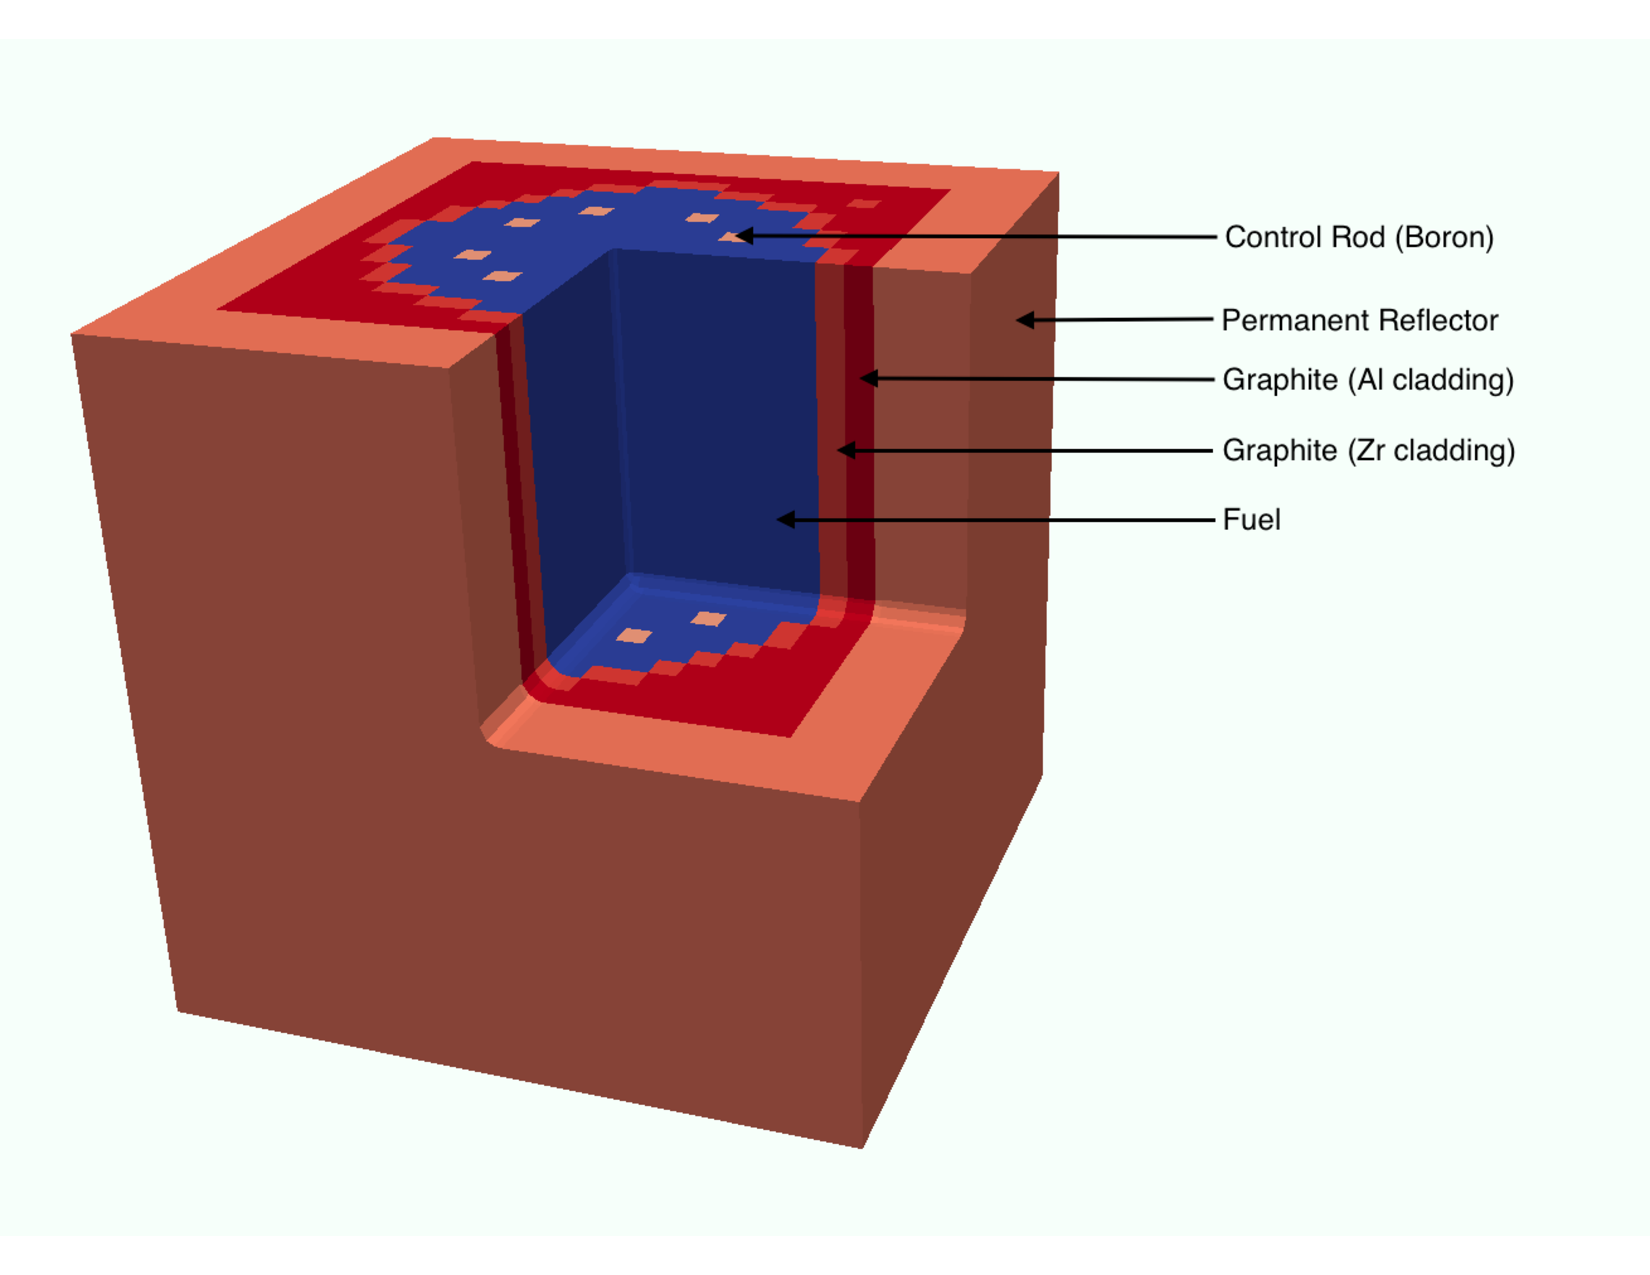
\includegraphics[scale=0.3]{./figures/transient-15.pdf}
 % \caption{Geometry of the Transient-15 model. \label{fig:treat_macro}}
}
\subfigure[Reactor Power Trace]
{
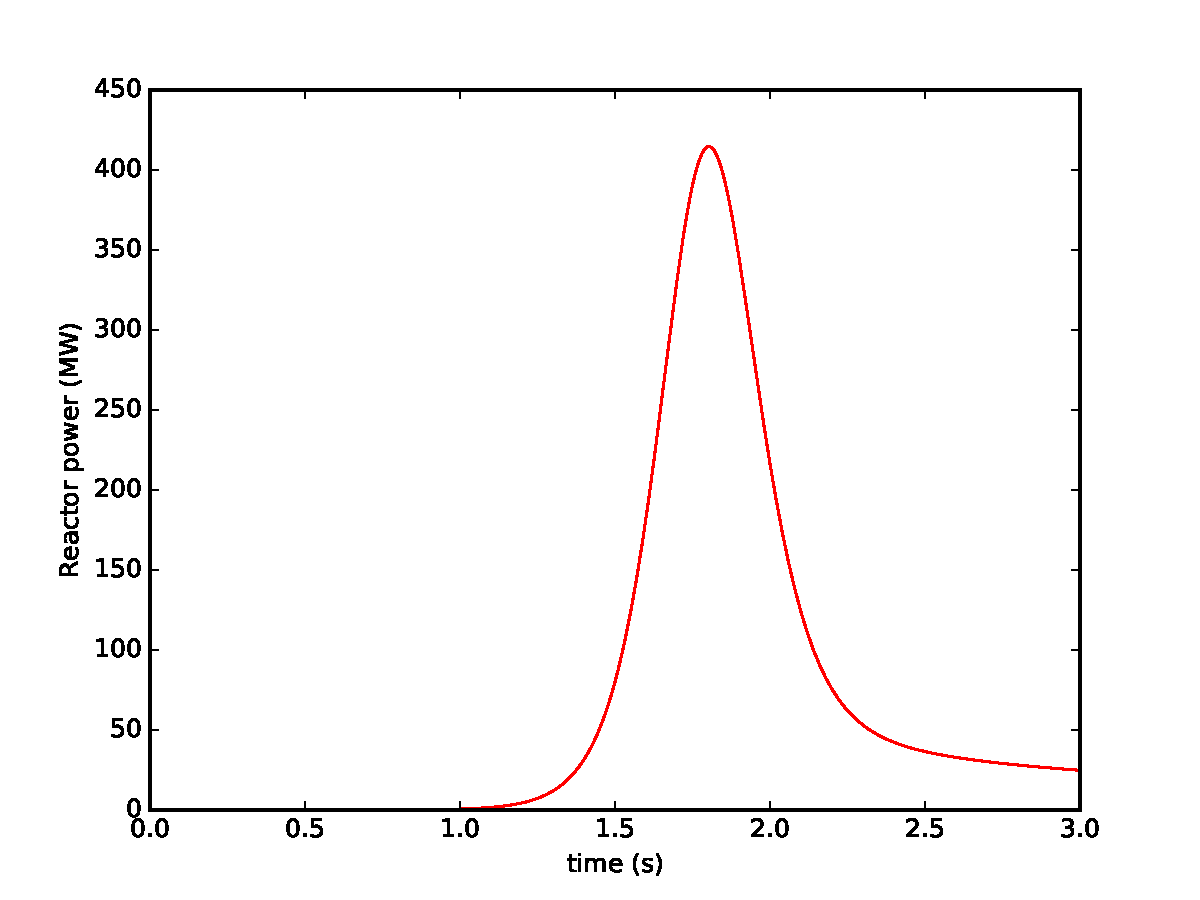
\includegraphics[scale=0.4]{./figures/transient-15_reactor_power.pdf}
 %
}
\caption{(a) Geometry of the Transient-15 model and (b) reactor power trace. \label{fig:treat_macro}}
\end{figure*}

%A trace of the integrated reactor power versus time is depicted in Fig. \ref{}.

%%%%%%%%%%%%%%%%%%%%%%%%%%%%%%%%%%%%%%%%%%%%%%%%%%%%%%%%%%%%%%%%%%%%%%%%%%%%%%%%
\subsection{Microscopic UO2 pellet - Graphite model}\label{sec:micro_model}
Micro-structure models are created for two points within the domain referred to as P1 and P2: point P1 at the center $\vec{r} = (0, 0, 125.74)$ cm and point P2 at $\vec{r} = (40.75, 20.5, 180)$ cm slightly more elevated and within a control rod region, cf. Fig. \ref{fig:treat_macro}. They are executed using MOOSE's flexible Multiapp system that allows spawning sub-applications from the master application \cite{Multiapp}.
The micro-structure model comprises three isotopes: $^{12}C$ in the region outside of the fuel grain, $^{235}U$ and $^{16}O$ within the fuel grain. Note that this composition resembles the HEU core, while in the LEU core the majority of uranium will be $^{238}U$ creating potentially different fission products.
For avoiding Gibbs' phenomenon when projecting the concentration values onto an FEM mesh, it is essential to ensure a smooth transition of the concentration from one region to another. For this purpose, MOOSE's SmoothSuperellipsoidIC are used allowing for a smooth transition of the concentration value within the grain to the outside value. An additional variable $\theta$ is defined that is $1$ within the fuel grain and $0$ outside the fuel grain.
Fuel grains are conjectured to be shaped more like "corn flakes" \cite{Mark}, \cite{GraphiteCore}, as opposed to spheres. To explore the impact of the fuel grain's shape two cases are considered: (1) a spherical fuel grain with radius $20 \mu m$, and (2) a ellipsoidal grain with semi-axes $a=b=31.748 \mu m$ and $c=7.937 \mu m$ yielding an aspect ratio of four.

We are interested in determining the microscopic distribution of the heat source $q'''$. The fission rate $f$, i.e. the number of fissions per time and unit volume, that a single fuel grain experiences is given by:
\begin{equation}
  f = \frac{P}{\kappa Q r},
\end{equation}
where $P$ is the local power density transferred from the macroscopic solve, $\kappa$ is the fuel volume fraction $\kappa = 1 : 2571 \approx 0.0004$ \cite{Mo2015}, Q is the energy released per fission taken as $192.9$ MeV \cite{DH}, and $r$ is an arbitrary scaling factor for controlling the number of PKAs. The fission rate $f$ is used to sample the number of fission events and hence PKAs. The energy deposited by the fission fragments and secondaries within a given timestep is denoted by $E_{D}(\vec{r}, t)$.
The total energy deposited at position $\vec{r}$ and time $t$ is:
\begin{equation}
   q'''(\vec{r},t) = r \frac{E_D(\vec{r},t)}{\Delta t} + \tau P,
\end{equation}
where $\tau$ is the fraction of energy released as anything but fission fragments, $\tau = 13.2$ \%, \cite{DH}.

The heat source is then used to drive the heat-conduction problem:
\begin{align}\label{eq:micro_heat}
   \frac{\partial (\rho c_p(T) T)}{\partial t}& - \nabla \cdot k(T) \nabla T = q''' \text{ on }D, \nonumber \\
    T(0) &= 300, \nonumber \\
     \nabla T \cdot \vec{n} &=0\text{ on } \partial D,
\end{align}
where the density $\rho$, the specific heat capacity $c_p(T)$, and the thermal conductivity $k(T)$ are taken from \cite{Mo2015}. We assume no degradation due to irradiation [neglect Eq. (3) in \cite{Mo2015} and only use Eq. (1) and (2)]. The domain $D$ is chosen to be $(400~\mu m)^3$ and is initially covered by a uniform 50x50x50 quadrilateral mesh that is adaptively refined 3 times at the graphite fuel interface.

\subsection{Numerical Results}
In the first part, the heat source is characterized for a spherical fuel particle at the center of the TREAT reactor, and in the second part solutions to the heat conduction problem Eq. \eqref{eq:micro_heat} are presented for points P1 and P2 and spherical and ellipoidal fuel grains.

\subsubsection{Heat Source Characterization}
We consider a spherical fuel particle of radius $r=20\mu m$ located at the center of the transient 15 TREAT core \cite{Ortensi2015}. The heat source depicted in Fig. \ref{fig:heat_source} is a snap shot at roughly $t=2$ seconds into the transient putting it close to the peak power. Figure \ref{fig:heat_source} depicts averages over spherical shells centered about the fuel grain's center.
At the selected time TREAT's total power is $312$ MW and the macroscopic power density at the selected point is $p(\vec{r_f}, t=2) = 262.9$ $\text{W}/ \text{cm}^3$. The microscopic distribution of power is highly concentrated in the fuel grain reaching $0.5$ $\text{MW}/ \text{cm}^3$ and a significant fraction of the energy is deposited within a distance of 10 $\mu m$ of the fuel grain in the graphite matrix. The reason for the large power density is that the fuel grain only assumes a very small fraction of the total volume, but receives most of the energy deposition from fission fragments. As we move away from the center of the fuel particle, the asymptotic value of the heat source is $\lim\limits_{r\rightarrow \infty} q''' = 41.5$ W.

The fit of the heat source in the fuel uses an even polynomial of fourth order, and the moderator power uses a complete fourth order polynomial. The choice of the polynomial in the fuel originates from the observation that the
heat source should be symmetric about $r=0$. As the volume for small $r$ is significantly smaller than for large $r$ the corresponding data points exhibit strong statistical fluctuations.

\begin{figure}[ht] % replace 't' with 'b' to force it to be on the bottom%
 \centering
  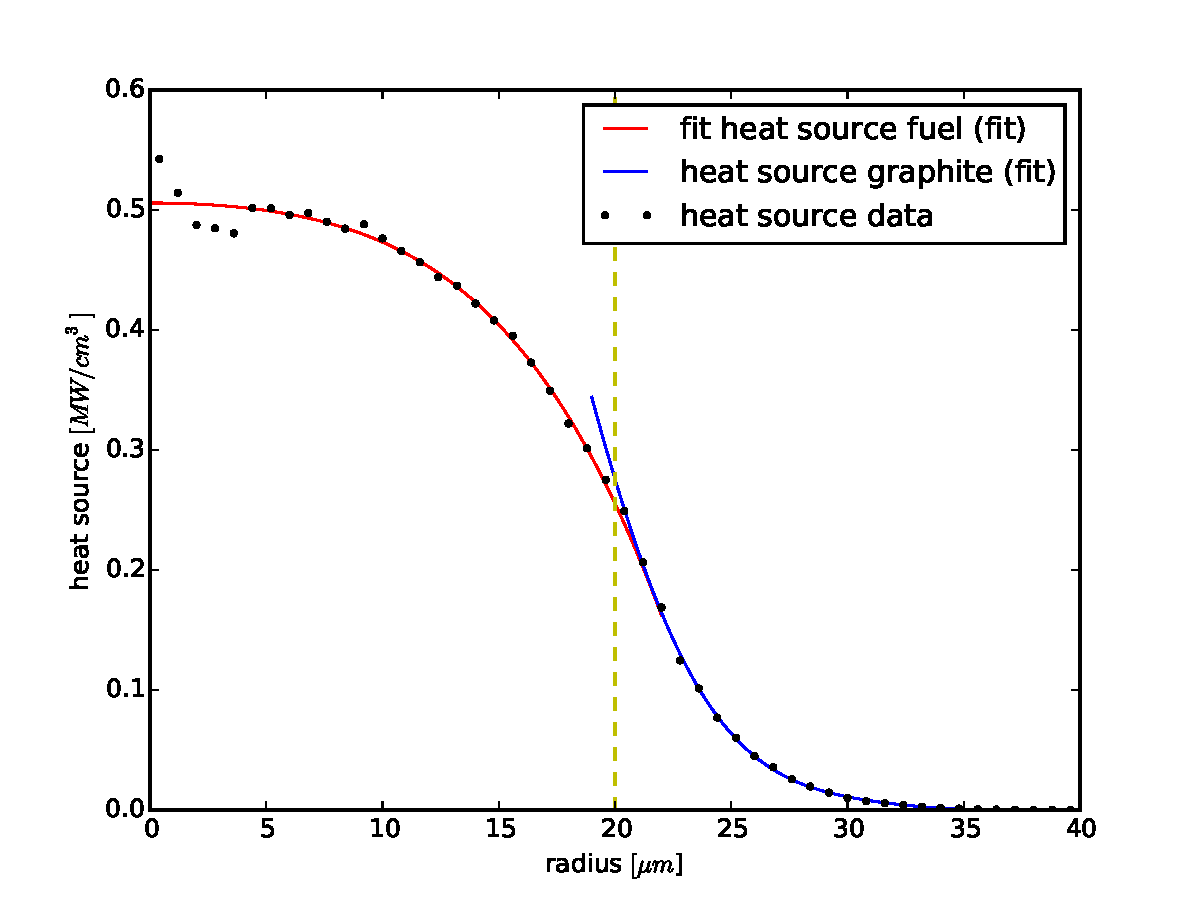
\includegraphics[scale=0.45]{./figures/heat_source.pdf}
  \caption{Heat source for a spherical fuel particle of radius $r=20 \mu m$ at the center of the TREAT transient 15 core at a total power of $312$ MW. \label{fig:heat_source}}
\end{figure}

\subsubsection{Microscopic Temperature Distribution}
The heat equation Eq.~\eqref{eq:micro_heat} is advanced in time at the end of each macroscopic timestep first recomputing the heat source distribution using BCMC and then advancing Eq.~\eqref{eq:micro_heat} in time. We do not allow sub-cycling so the sub-application timestep is set equal to the master's timestep $\Delta t = 0.01$ and the Crank-Nicolson time integrator is used.

Within this manuscript we are interested in the average fuel and graphite temperatures defined as:
\begin{align}
  T_f(t) &= \frac{\int\limits_{D} \theta(\vec{r}) T(\vec{r}, t) dV }{\int\limits_{D} \theta(\vec{r}) dV} \nonumber \\
     T_g(t) &= \frac{\int\limits_{D} (1 - \theta(\vec{r})) T(\vec{r}, t) dV }{\int\limits_{D} (1 - \theta(\vec{r})) dV},
\end{align}
which will be a good measure of the respective feedback that can be expected from the graphite and, in the LEU case, from
the fuel. Given the power trace depicted in Fig. \ref{fig:treat_macro} (b), the traces for fuel and graphite temperature for a spherical grain and ellipsoidal grain are depicted in Fig. \ref{fig:micro_heat_cond} (a) and (b), respectively.

As previously observed in \cite{Mo2015}, the fuel temperature peaks shortly after TREAT reaches maximum power. At this point, the graphite has not sufficiently heated up and hence acts as strong enough heat sink to reduce the fuel temperature until both graphite and fuel temperatures have equilibrated sufficiently to allow $T_f$ to increase again. As time progresses and the reactor power stabilizes, the difference between $T_g$ and $T_f$ approaches a constant value close to zero. The fuel and graphite temperature as well as the difference between fuel and graphite temperature is larger at P1 than at P2 because of the larger local power density.

The first important finding of this work is that the shape of the fuel grain has a small but measurable effect on the average fuel temperature but no effect on the moderator temperature. The graphite temperature traces remain unchanged when moving from the spherical to the ellipsoidal fuel grain, while the peak fuel temperature in the spherical case is roughly $10$ K and $5$ K higher than in the ellipsoidal case for P1 and P2, respectively. It is intuitively clear that the graphite temperature remains unchanged due to the large amount of graphite and small amount of fuel in the computational cell. We can estimate the order of magnitude of change in reactivity attributed to these temperature difference if they applied uniformly throughout the core [which of course they do not as they are space-depend; however this exercise is still insightful]. Assuming the Doppler feedback coefficient to be $10^{-5}$ and using $\beta \approx 0.007$ obtained from the TREAT cross section data, $10$ K difference in fuel temperature translates to a reactivity worth of $1.5$ cents in LEU fuel. This reactivity change is expected to be larger for high-power transients because of an expected increase in temperature difference between spherical and ellipsoidal shapes.

Secondly, the temperature difference between fuel and graphite is quite significant at point P1: $80$ K and $70$ K for the spherical and ellipsoidal case at the fuel temperature's peak, respectively; at point P2 the difference is much smaller, $\approx20$. If the model had not accounted for the difference in fuel and graphite temperature, i.e. set $T_f = T_g$, we would miss about $10-11$ cents of reactivity if the temperature difference at P1 applied everywhere in the core. Using the data at P2 leads to a smaller negative reactivity of about $2-3$ cents; the overall system response would be an importance weighted average across the reactor core and could be elucidated with a fully coupled, multi-physics, multi-scale model. The difference in graphite and fuel temperature increases with increasing the reactor power and shortening the pulse, and hence in scenarios such as the EOS-2 transient in \cite{Mo2015} a significantly higher negative feedback is expected. This underpins the importance of taking into account the microscopic structure of TREAT fuel for a potential LEU conversion.

%%%%%%%%%%%%%%%%%%%%%%%%%%%%%%%%%%%%%%%%%%%%%%%%%%%%%%%%%%%%%%%%%%%%%%%%%%%%%%%%
\section{Conclusions and Future Work}
Within this work we describe a first step of multi-scale, multi-physics modeling of TREAT with particular emphasis on accurate heat source characterization around a TREAT fuel grain. To this end, we use a BCMC model that is coupled to an FEM application by the Magpie application to characterize the heat source of the micro-structure heat-conduction problem. The BCMC is driven by a macroscopic Rattlesnake, \cite{Rattlesnake}, neutronics calculation of TREAT transient 15. ENDF fission yield data is utilized for sampling PKAs. We present the shape of the heat source for a spherical fuel grain demonstrating that it significantly deviates from both a uniform distribution and a uniform distribution within the fuel grain and zero outside. The heat source is used to drive a microscopic heat conduction calculation resolving the fuel grain, either spherical [20 $\mu m$] or ellipsoidal in shape [aspect ratio of four and identical volume], from the graphite matrix. Both the average fuel and graphite temperatures are examined for the spherical and ellipsoidal fuel grain and put in perspective to the expected reactivity worth in case LEU fuel was used. It is found that the fuel temperature even in the case of the low-power transient 15 exceeds the graphite temperature by 80 K leading to an approximate reactivity difference of $11$ cents. This difference is expected to be larger for higher power and/or shorter transients. This underpins the need for multiscale simulation of a potential LEU core in order to ensure accurate account of the temperature feedback.

\begin{figure*}[t!] % replace 't' with 'b' to force it to be on the bottom%
\subfigure[Spherical Fuel Grain]
{
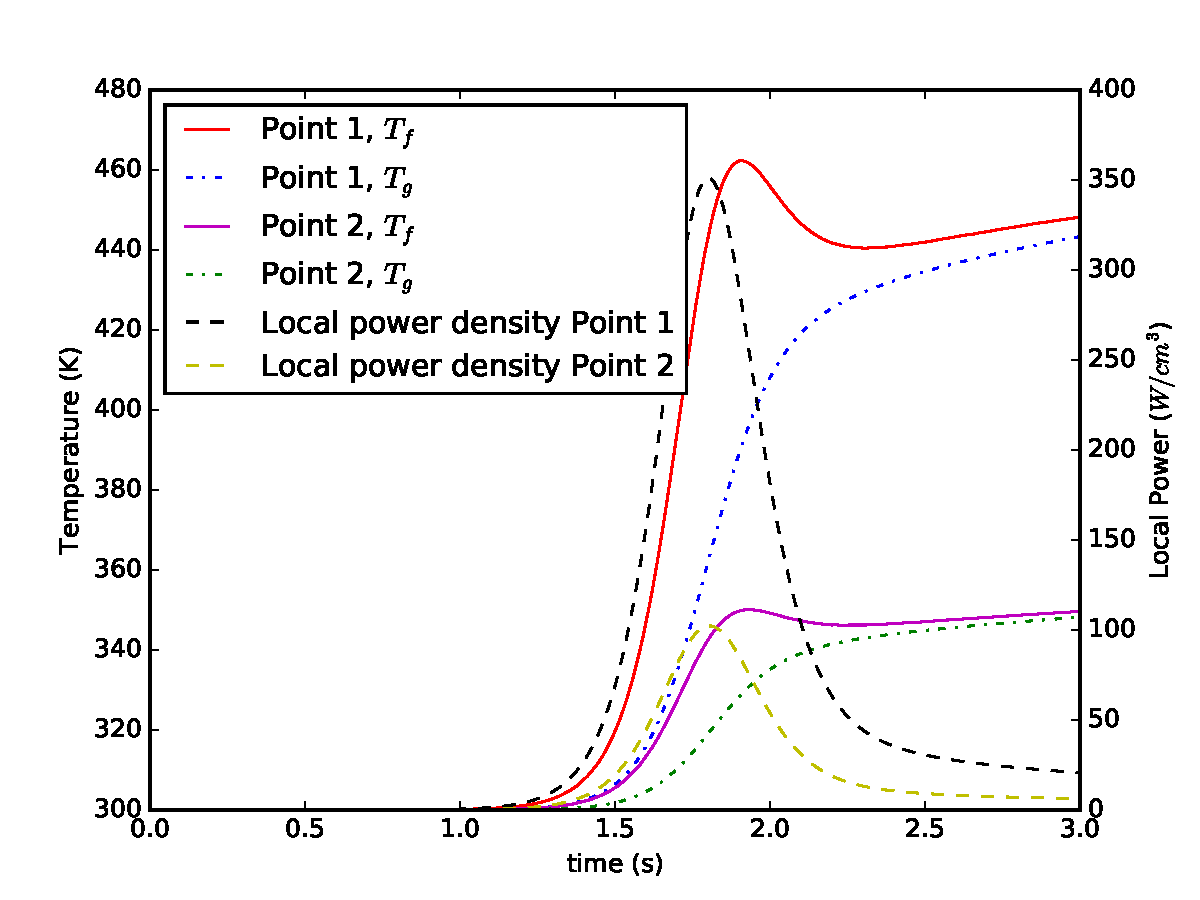
\includegraphics[scale=0.4]{./figures/spherical.pdf}
 % \caption{Geometry of the Transient-15 model. \label{fig:treat_macro}}
}
\subfigure[Ellipsoidal Fuel Grain]
{
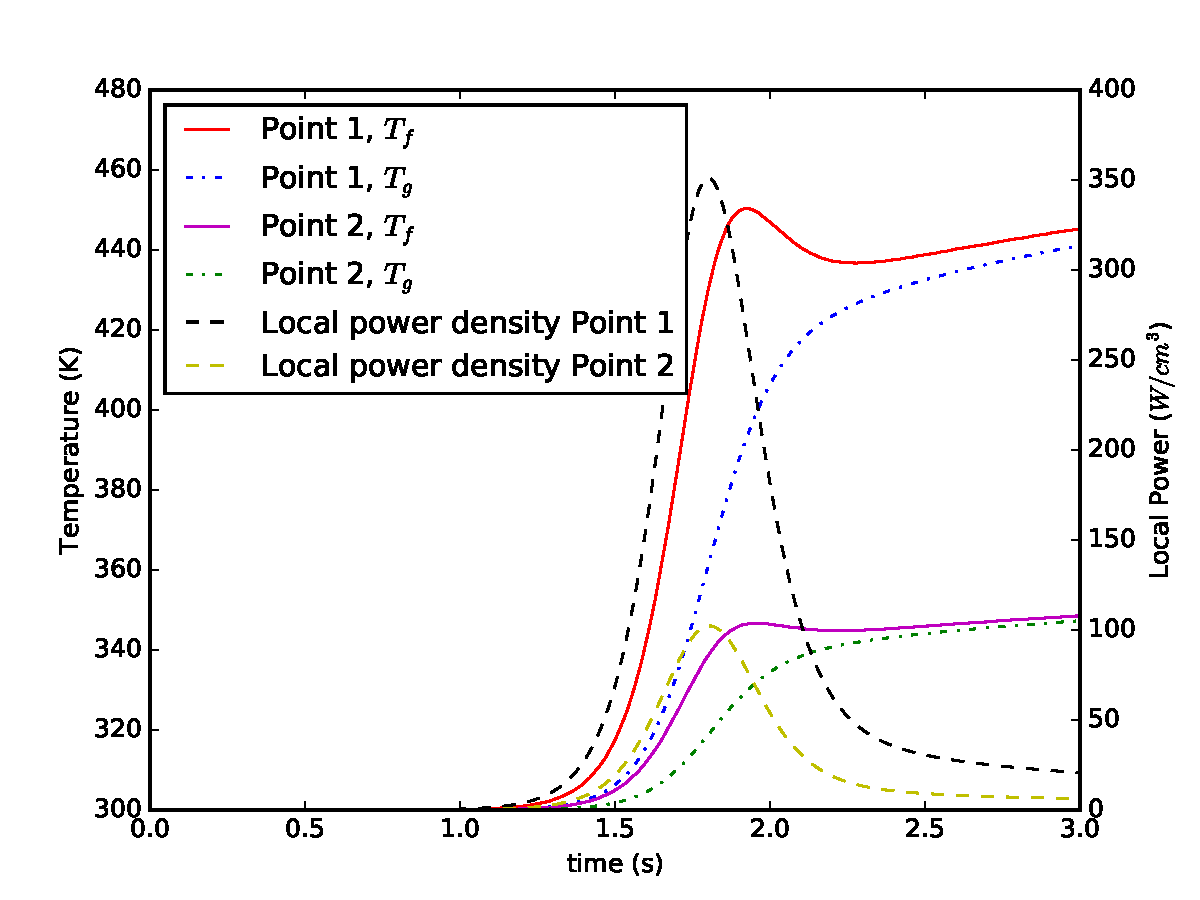
\includegraphics[scale=0.4]{./figures/ellipsoid.pdf}
 %
}
\caption{Evolution of microscopic average fuel and graphite temperatures for points P1 and P2 for spherical and ellipsoidal fuel grain shapes. \label{fig:micro_heat_cond}}
\end{figure*}

%%%%%%%%%%%%%%%%%%%%%%%%%%%%%%%%%%%%%%%%%%%%%%%%%%%%%%%%%%%%%%%%%%%%%%%%%%%%%%%%
%\clearpage
\section{Acknowledgments}
This work is supported by the U.S. Department of Energy, under DOE Idaho Operations Office Contract DE-AC07-05ID14517. Accordingly, the U.S. Government retains a nonexclusive, royalty-free license to publish or reproduce the published form of this contribution, or allow others to do so, for U.S. Government purposes.

%%%%%%%%%%%%%%%%%%%%%%%%%%%%%%%%%%%%%%%%%%%%%%%%%%%%%%%%%%%%%%%%%%%%%%%%%%%%%%%%
\begin{thebibliography}{1}

\bibitem{treat} U.S. Department of Energy, {\em Mission Need Statement for the Resumption of Transient Fuel Testing}, U.S. DOE, December 3, 2010.

\bibitem{Mo2015} Kun Mo et al., {\em Heat transfer simulations of the UO2 particle-graphite system in TREAT fuel}, Nuclear Engineering \& Design, Vol. 293, November, 2015.

\bibitem{TreatFeedback} Javier Ortensi et al.,  {\em Full Core TREAT Kinetics Demonstration Using Rattlesnake/BISON Coupling Within MAMMOTH}, Research report INL/EXT-15-36268, Idaho National Laboratory, Idaho Falls, Idaho, August 2015.

%\bibitem{GammaHeating} Y.K. Lee, J.-C. David, and H. CarCreff, {\em A Gamma Heating Calculation Methodology for Research Reactor Applications}. in Proc. 5th ENS Int.Topical Meeting Research Reactor Fuel Management, Aachen, Germany, Apr. 1-3, 2001.\\

\bibitem{SRIM} J. F. Ziegler and J. P. Biersack and M. D. Ziegler (2008). SRIM - The Stopping and Range of Ions in Matter. SRIM Co. ISBN 0-9654207-1-X.

\bibitem{COMSOL} {\em COMSOL Multiphysics 4.3b,} User's guide, COMSOL Inc.

\bibitem{Moose} H. Park, D. Knoll, D. Gaston, and R. Martineau, {\em Tightly Coupled Multiphysics Algorithms for Pebble Bed Reactors,} Nuclear Science and Engineering, Vol. 166(2), pp. 118-133, 2010.

\bibitem{MyTRIM} Daniel Schwen et al., {\em Molecular dynamics simulation of intragranular Xe bubble re-solution in UO 2}, Journal of Nuclear Materials, Vol. 392, 2009.

\bibitem{MAMMOTH} Mark DeHart, {\em TREAT Modeling and Simulation Development with Validation Requirements} Research report INL/CON-15-36200, Idaho National Laboratory, Idaho Falls, Idaho.

%\bibitem{basics} Mark T. Robinson, {\em Basic physics of radiation damage production}
%Journal of Nuclear Materials 216 (1994) 1-28 \\
%
%\bibitem{BCA} R. Smith (ed.) {\em Atomic and ion collisions in solids and at surfaces:
% theory, simulation and applications}, Cambridge University Press, Cambridge, UK,
%  1997 \\

\bibitem{ENDFManual} The Members of the Cross Sections Evaluation Working Group, {\em ENDF-6 Formats Manual}, Research Report, Brookhaven National Laboratory,
BNL-90365-2009, Upton, NY, June, 2009.

\bibitem{geant} GEANT4 Physics Manual Version: 10.2 (4 December 2015).

\bibitem{Ortensi2015} J. Ortensi, M. D. DeHart, F. N. Gleicher, Y. Wang, A. L. Alberti and T. S. Palmer, {\em Full Core TREAT Kinetics Demonstration Using Rattlesnake/BISON Coupling Within MAMMOTH}, INL/EXT-15-36268, Idaho National Laboratory, Idaho Falls, Idaho, September 2015.

\bibitem{Mark} Personal Communication with Mark DeHart.

\bibitem{GraphiteCore} M.W. Davies, {\em Graphite Core Design in UK Reactors}, Technical Report, National Nuclear Corporation, XA9642901.

\bibitem{averagedistance} Bhattacharyya, P., and B. K. Chakrabarti. The mean distance to the nth neighbour in a uniform distribution of random points: an application of probability theory. Eur J. Phys. 29, pp. 639-645.

\bibitem{DH} James J. Duderstadt and Louis J. Hamilton, {\em Nuclear Reactor Analysis}, John Wiley \& Sons, 1976.

\bibitem{Rattlesnake} Y. Wang et al., {\em Rattlesnake: User Manual}, Technical Report, Idaho National Laboratory, Idaho Falls, ID, 2016.

\bibitem{Multiapp} Y. Wang et al., {\em Rattlesnake: User Manual}, Technical Report, Idaho National Laboratory, Idaho Falls, ID, 2016.

\end{thebibliography}



\end{document}
